\section{Istruzioni per l'uso}
\subsection{Requisiti di sistema}
Il server$_G$ ospitante l'applicazione dovrà soddisfare alcuni requisiti di seguito elencati:
\begin{itemize}
\item Sistema operativo Ubuntu$_G$ 14.04 LTS o Mac OSX v.10 o superiore;
\item Browser Google Chrome$_G$ v.40 o superiore;
\item Disco rigido con almeno 250,0 MB di memoria disponibili.
\end{itemize}

\section{Files necessari}
Per procedere all'installazione dell'applicazione \emph{Premi} sono necessari alcuni file contenenti il codice sorgente.
Tali file sono reperibili all'interno del repository$_G$ pubblico all'indirizzo \href{http://404notfoundunipd.github.io/premi/}{http://404notfoundunipd.github.io/premi/}, dove si troveranno tutte le istruzioni necessarie per scaricare i file dell'applicazione.

\section{Installazione}
\subsection{Linux e Mac OS}

\subsubsection{Installazione curl}
Curl è uno strumento per riga di comando e libreria per il trasferimento di dati con sintassi URL$_G$. \\

\noindent Per eseguire l'installazione aprire il terminale e digitare in sequenza i seguenti comandi (solo Ubuntu$_G$ o derivati Debian$_G$):

\begin{lstlisting}[style=DOS]
	$ sudo apt-get update
	$ sudo apt-get install libcurl3
\end{lstlisting}

\noindent Alternativamente è possibile eseguire l'installazione scaricando il pacchetto d'installazione dal sito \href{http://curl.haxx.se/download.html}{http://curl.haxx.se/download.html}; una volta scaricato il pacchetto, estrarne i file in una cartella come nell'immagine seguente:

\begin{figure}[h]
\begin{center}
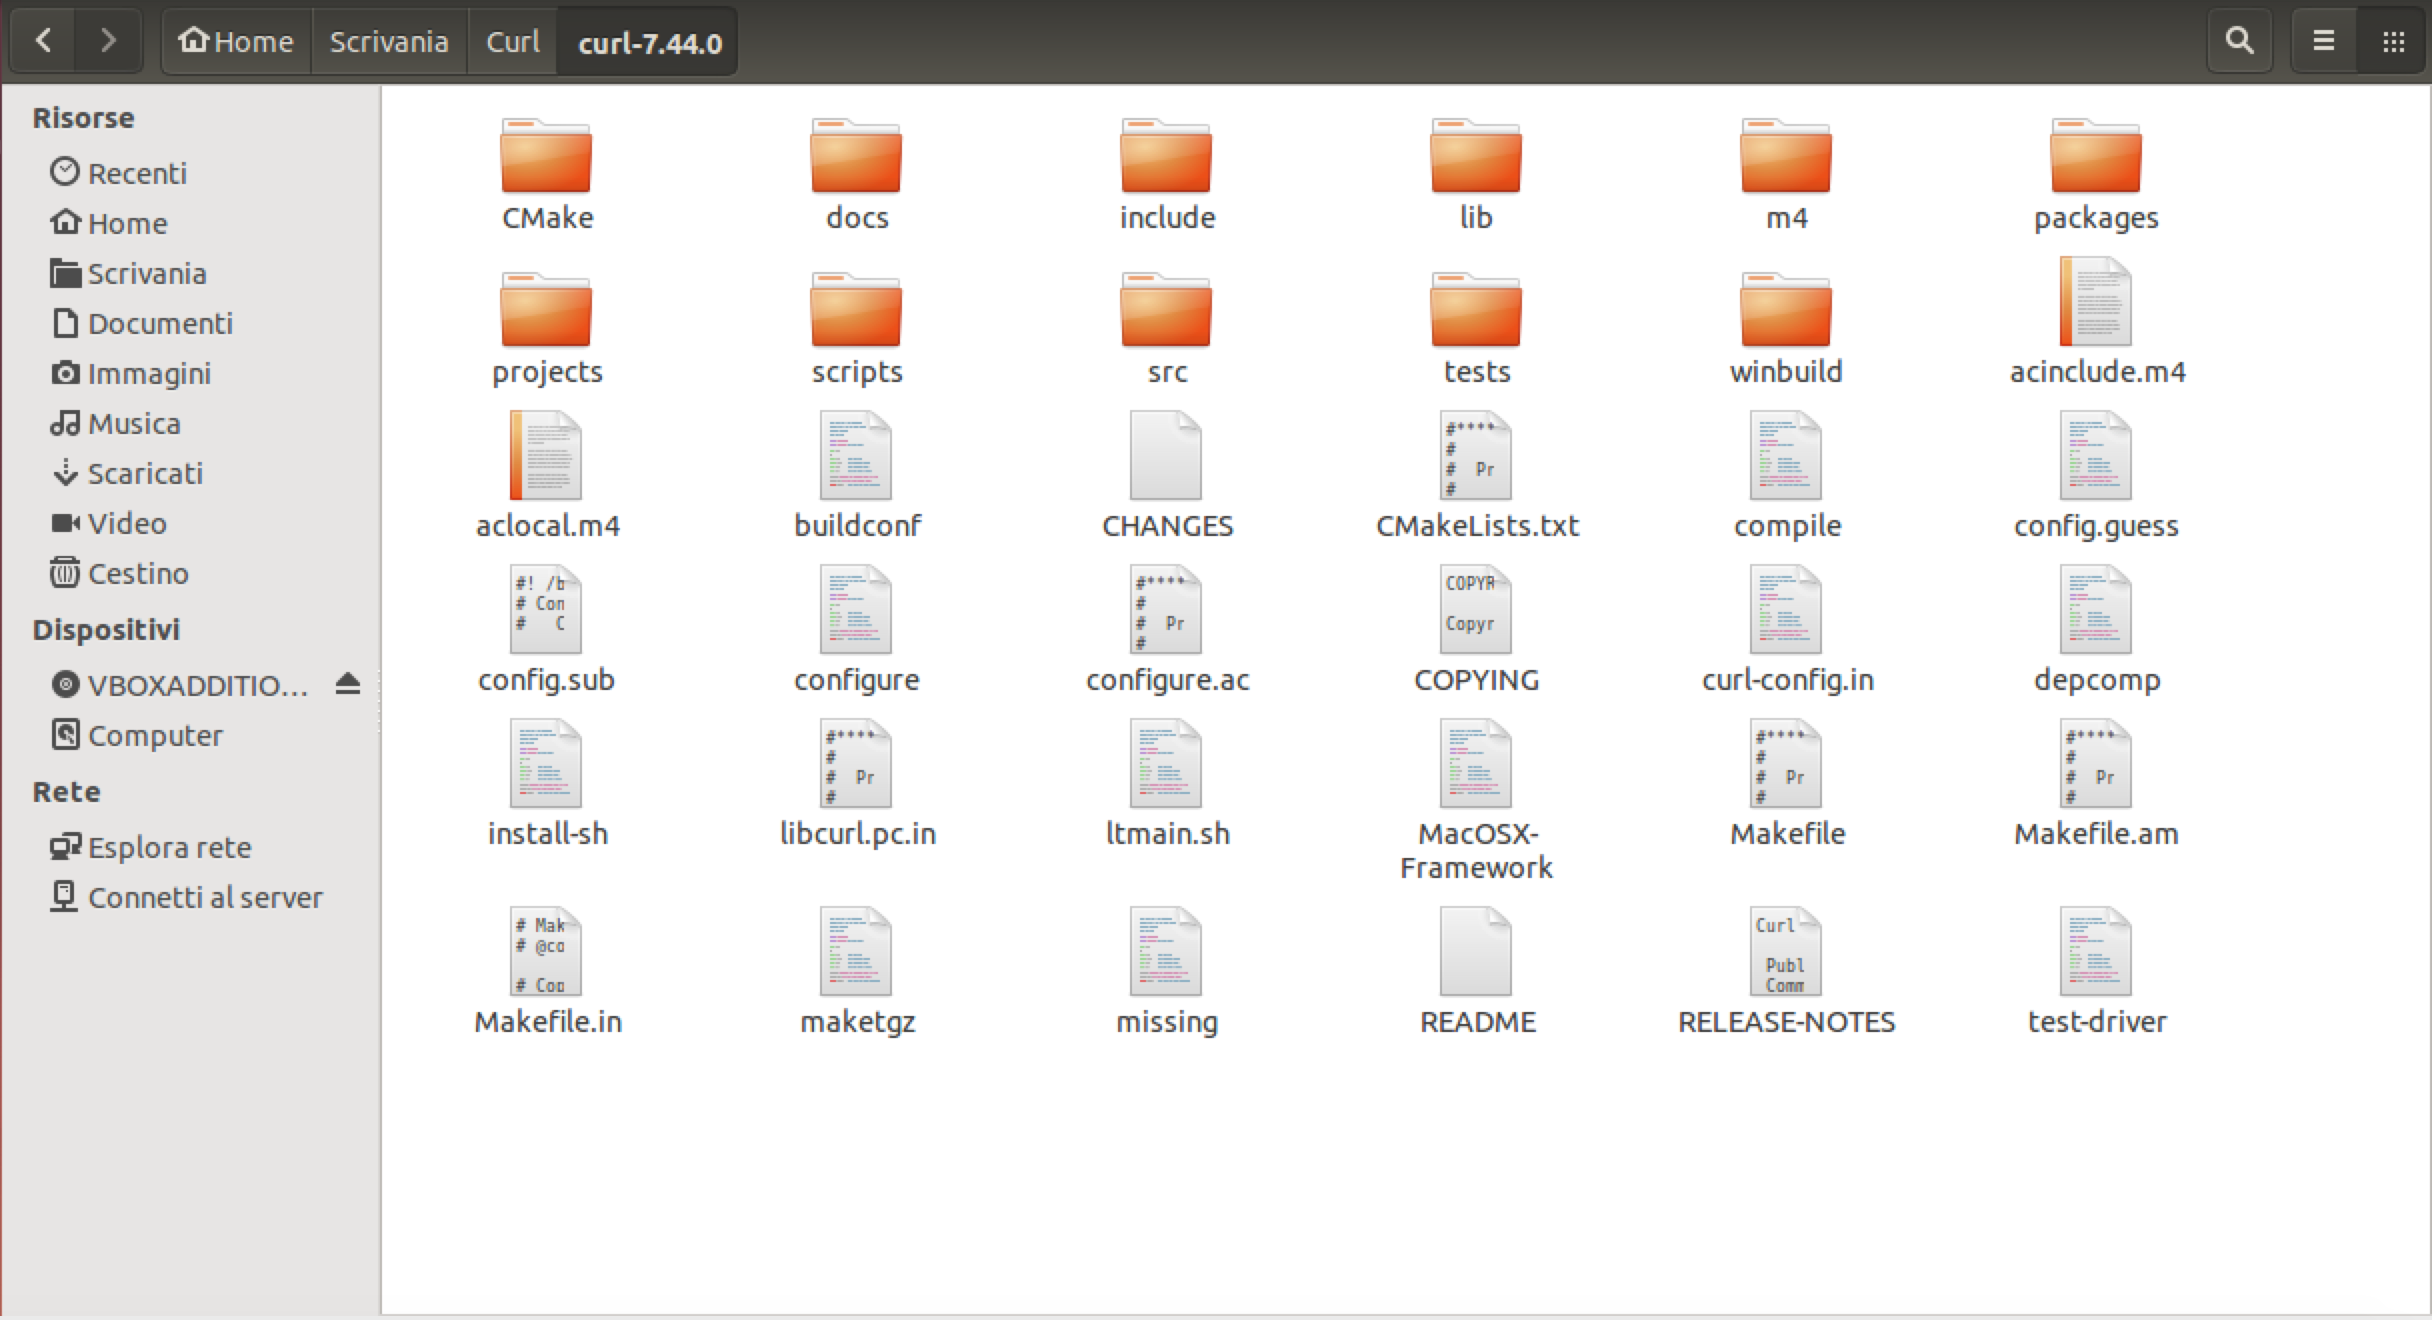
\includegraphics[scale=0.3]{img/curl_files_linux.png}
\caption{File \emph{curl} su ambiente linux.}
\end{center}
\end{figure}

\newpage
\noindent Supponiamo ora di avere estratto i file all'interno della cartella \\
\verb+/home/notfound404/Desktop/Curl/curl-7.44.0/+.\\
Aprire quindi il terminale e spostarsi all'interno di questa cartella tramite il comando:

\begin{lstlisting}[style=DOS]
	$ cd /home/notfound404/Desktop/Curl/curl-7.44.0/
\end{lstlisting}

\noindent eseguire quindi in sequenza i comandi:

\begin{lstlisting}[style=DOS]
	$ ./configure
	$ make
	$ make test (optional)
	$ sudo make install
\end{lstlisting}
Se la procedura è andata a buon fine \emph{curl} sarà stato installato correttamente.

\subsubsection{Installazione MeteorJS$_G$}
\emph{MeteorJS$_G$} è una piattaforma completamente Open Source$_G$ per lo sviluppo di applicazioni web o mobile in JavaScript.\\
Per eseguire la sua installazione sarà sufficiente aprire il terminale ed eseguire il comando:

\begin{lstlisting}[style=DOS]
	$ curl https://install.meteor.com/ | sh
\end{lstlisting}

\noindent Una volta terminata l'installazione, MeteorJS$_G$ sarà pronto per essere utilizzato.

\subsubsection{Avvio applicazione}
Dopo aver scaricato l'archivio contenente i files necessari, come spiegato nella sezione \emph{3 Files necessari}, è necessario scompattarlo estraendone i files in una cartella, che per comodità supponiamo essere \verb+/home/notfound404/Desktop/Premi/+.\\
Per avviare l'applicazione aprire il terminale, spostarsi all'interno della cartella con il comando

\begin{lstlisting}[style=DOS]
	$ cd /home/notfound404/Desktop/Premi/
\end{lstlisting}

\noindent e avviare MeteorJS$_G$ con il comando 

\begin{lstlisting}[style=DOS]
	$ sudo meteor
\end{lstlisting}

\begin{figure}[!h]
\begin{center}
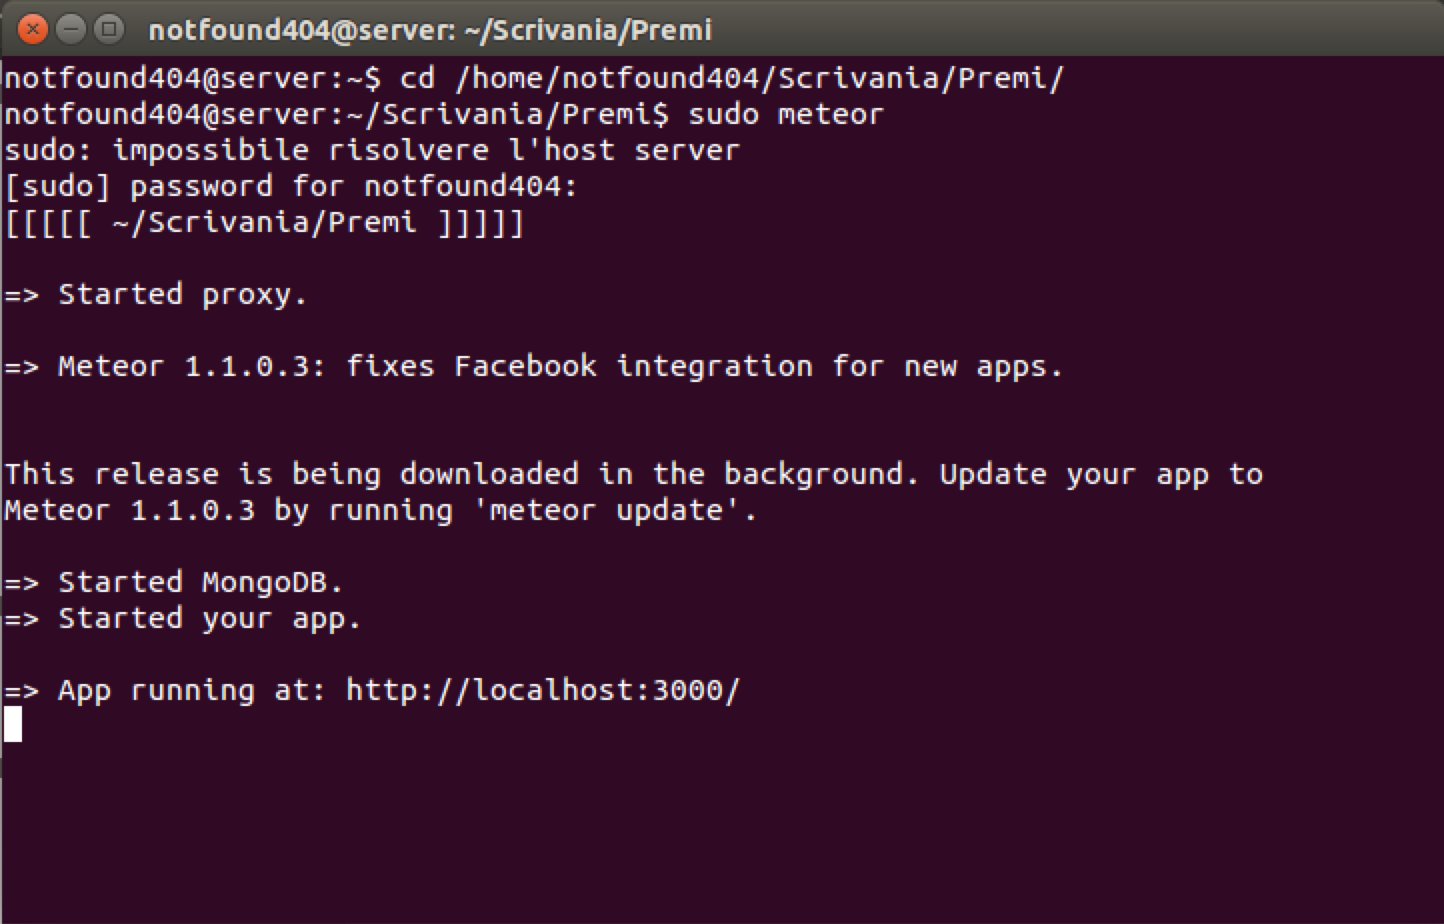
\includegraphics[scale=0.4]{img/start_premi.png}
\caption{Avvio applicazione.}
\end{center}
\end{figure}

\newpage
Nel caso vengano riscontrati errori verificare i seguenti punti:
\begin{itemize}
\item connettività ad internet; potrebbe essere necessario il download di alcuni pacchetti mancanti in seguito al primo avvio dell'applicazione;
\item controllare che all'interno della cartella \emph{Premi}, contenente i files dell'applicazione, sia presente anche la cartella \verb+.meteor+, sarà necessario abilitare la visualizzazione dei files nascosti;
\item verificare di disporre i privilegi di amministratore.
\end{itemize}

\noindent Nel caso in cui nessuna delle soluzioni sopra indicate porti ad una soluzione del problema, contattare gli sviluppatori attraverso le modalità indicate nella sezione \emph{1.5 Assistenza tecnica} del documento corrente.\\

\noindent Se invece l'applicazione è stata avviata correttamente verrà visualizzato sul terminale il messaggio 

\begin{lstlisting}[style=DOS]
	$ => App running at: http://localhost:3000/
\end{lstlisting}

\noindent Sarà quindi sufficiente aprire il browser$_G$ Google Chrome$_G$ ed inserire nella barra degli indirizzi \verb+http://localhost:3000/+ oppure \verb+http://127.0.0.1:3000/+.

\begin{figure}[!h]
\begin{center}
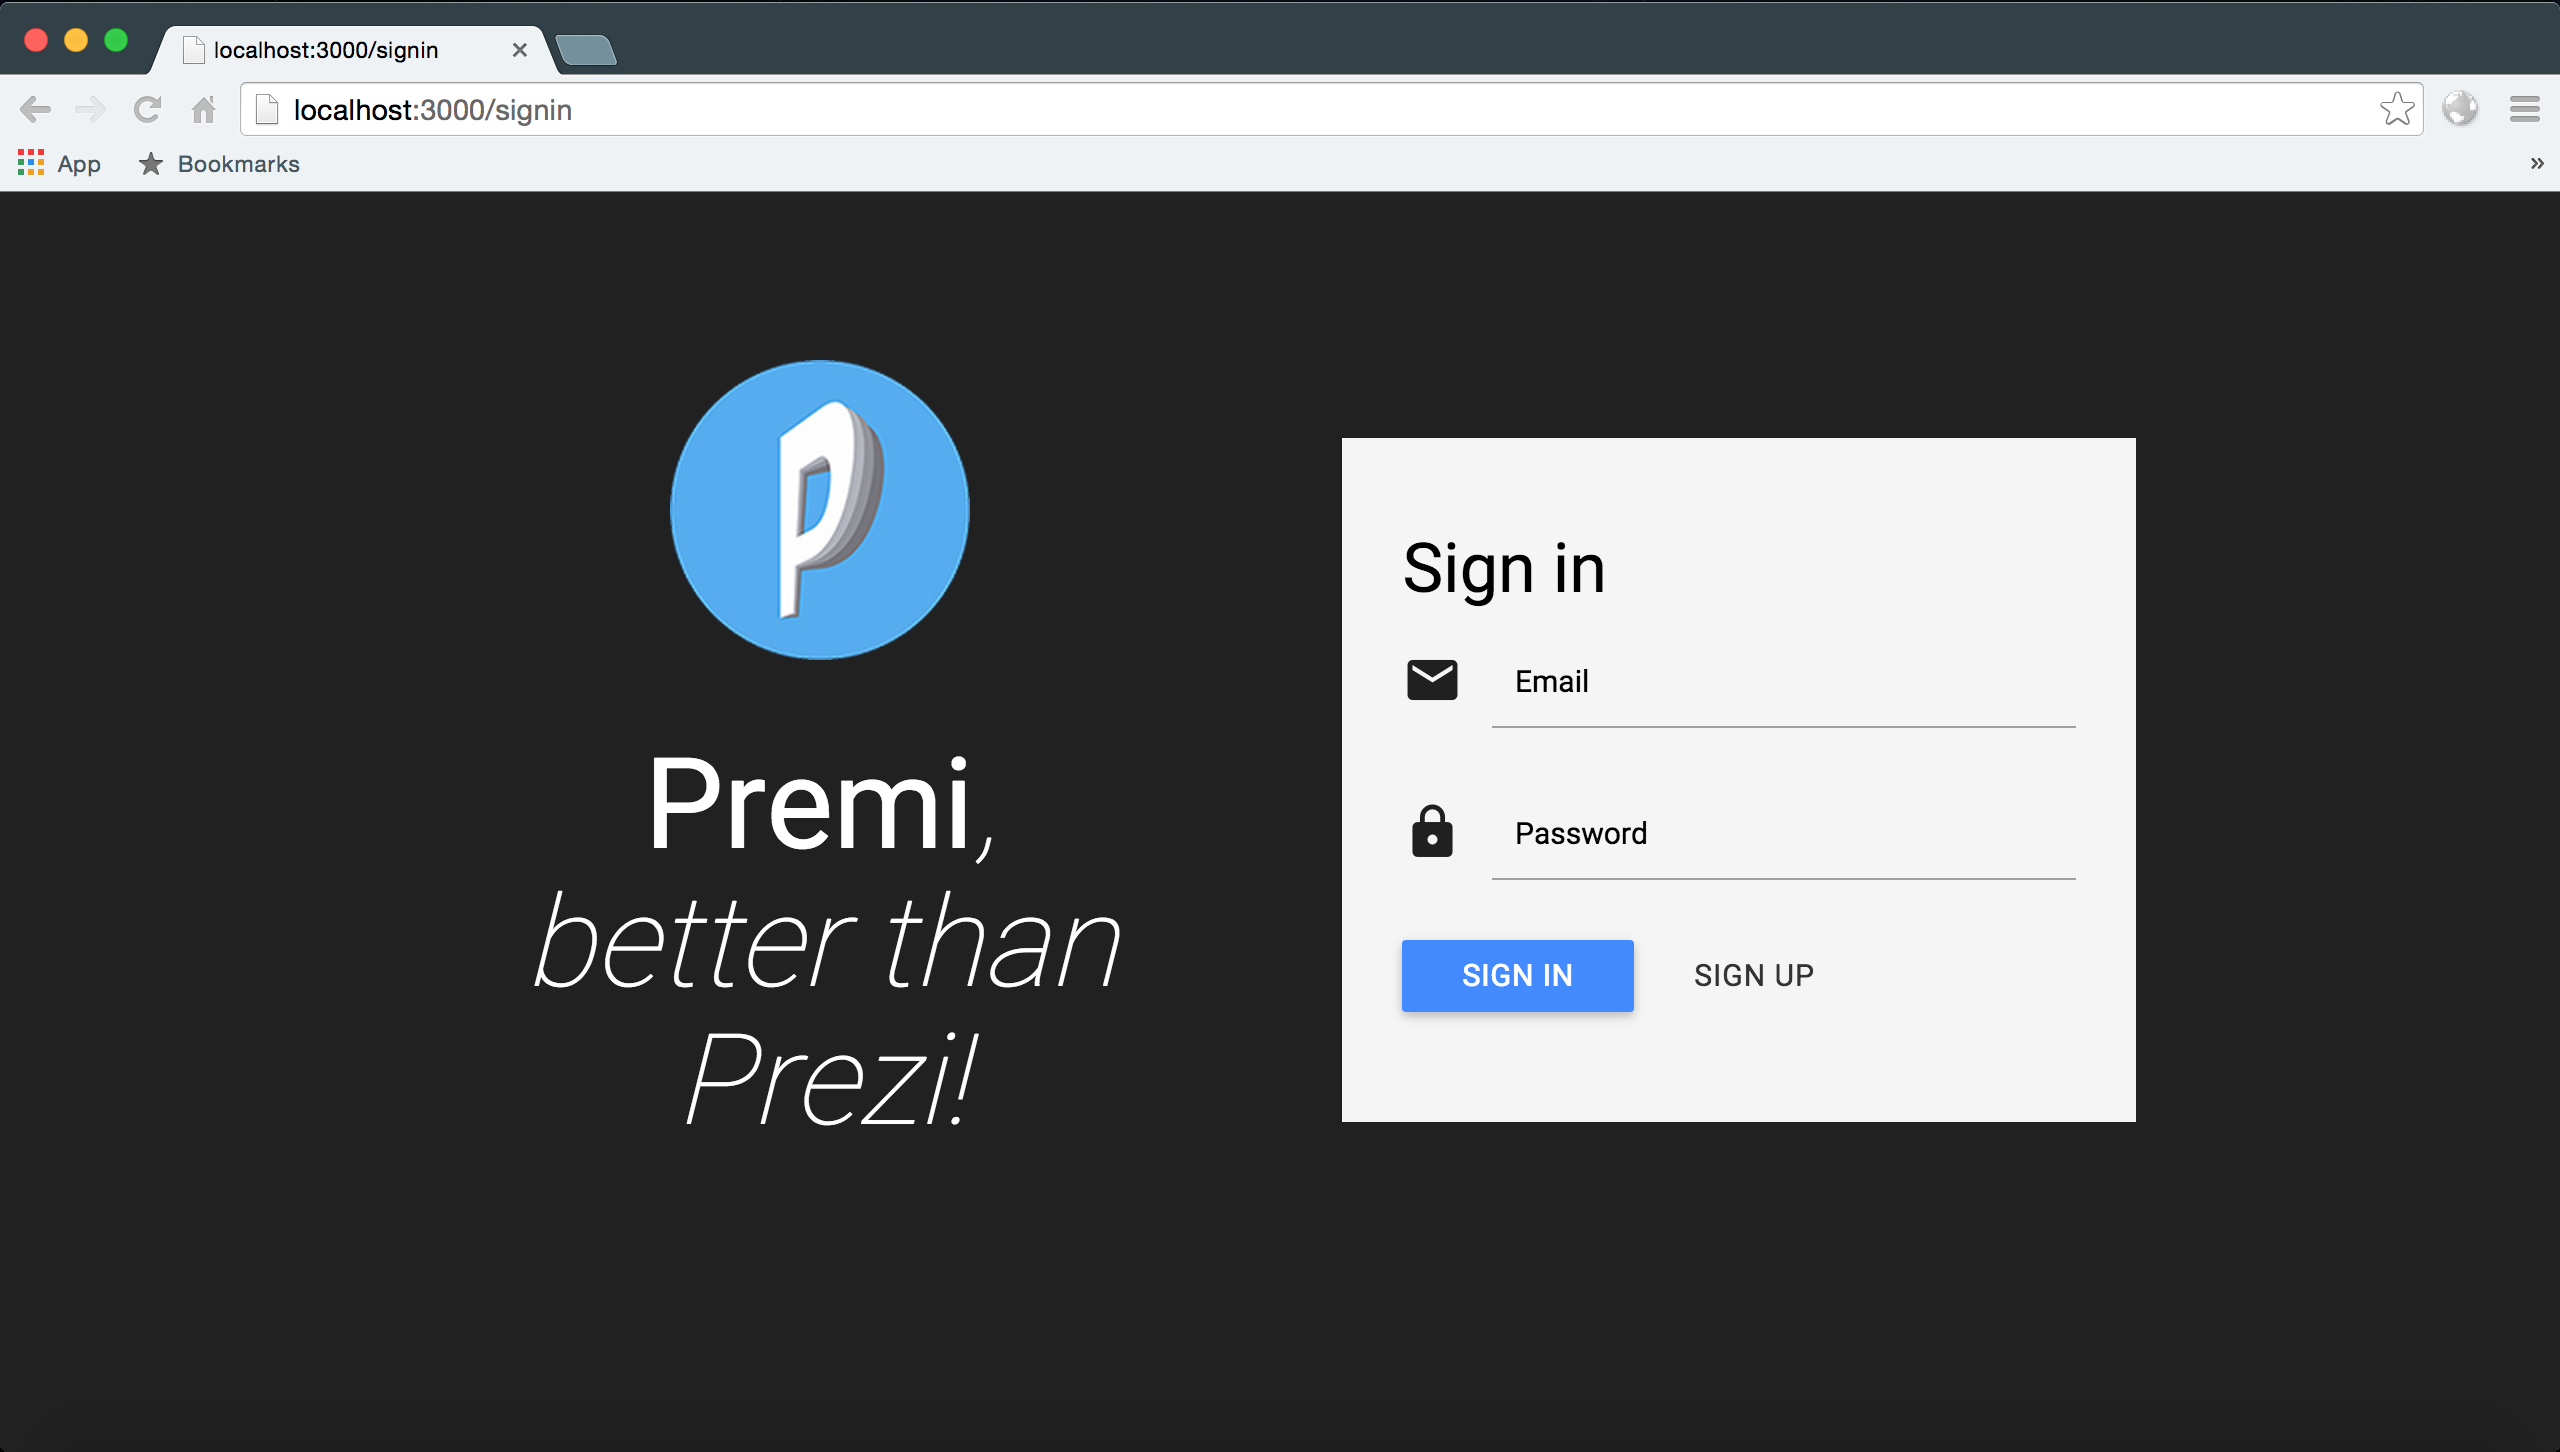
\includegraphics[scale=0.3]{img/app_started.png}
\caption{Avvio applicazione.}
\end{center}
\end{figure}

\noindent Per effettuare l'accesso all'applicazione tramite la rete, il server deve disporre di indirizzo IP pubblico e una corretta configurazione della propria rete.